%!TeX root=../wowtop.tex

	\ArtChapter[The Falling Star]{2head}





\lettrine[lines=4]{T}{hen} came the night of the first falling star. It was seen early in the morning, rushing over Winchester eastward, a line of flame high in the atmosphere. Hundreds must have seen it, and taken it for an ordinary falling star. Albin described it as leaving a greenish streak behind it that glowed for some seconds. Denning, our greatest authority on meteorites, stated that the height of its first appearance was about ninety or one hundred miles. It seemed to him that it fell to earth about one hundred miles east of him.

I was at home at that hour and writing in my study; and although my French windows face towards Ottershaw and the blind was up (for I loved in those days to look up at the night sky), I saw nothing of it. Yet this strangest of all things that ever came to earth from outer space must have fallen while I was sitting there, visible to me had I only looked up as it passed. Some of those who saw its flight say it travelled with a hissing sound. I myself heard nothing of that. Many people in Berkshire, Surrey, and Middlesex must have seen the fall of it, and, at most, have thought that another meteorite had descended. No one seems to have troubled to look for the fallen mass that night.

But very early in the morning poor Ogilvy, who had seen the shooting star and who was persuaded that a meteorite lay somewhere on the common between Horsell, Ottershaw, and Woking, rose early with the idea of finding it. Find it he did, soon after dawn, and not far from the sand-pits. An enormous hole had been made by the impact of the projectile, and the sand and gravel had been flung violently in every direction over the heath, forming heaps visible a mile and a half away. The heather was on fire eastward, and a thin blue smoke rose against the dawn.

%\begin{figure}[p]
%\centering
%
\includegraphics[width=\linewidth]{2fallenstar}
%\caption{Taken it for an ordinary falling star}
%\end{figure}

\begin{sidewaysfigure}

\includegraphics[width=\columnwidth]{2fallenstar}%
\caption{Taken it for an ordinary falling star}
\end{sidewaysfigure}

The Thing itself lay almost entirely buried in sand, amidst the scattered splinters of a fir tree it had shivered to fragments in its descent. The uncovered part had the appearance of a huge cylinder, caked over and its outline softened by a thick scaly dun-coloured incrustation. It had a diameter of about thirty yards. He approached the mass, surprised at the size and more so at the shape, since most meteorites are rounded more or less completely. It was, however, still so hot from its flight through the air as to forbid his near approach. A stirring noise within its cylinder he ascribed to the unequal cooling of its surface; for at that time it had not occurred to him that it might be hollow.

He remained standing at the edge of the pit that the Thing had made for itself, staring at its strange appearance, astonished chiefly at its unusual shape and colour, and dimly perceiving even then some evidence of design in its arrival. The early morning was wonderfully still, and the sun, just clearing the pine trees towards Weybridge, was already warm. He did not remember hearing any birds that morning, there was certainly no breeze stirring, and the only sounds were the faint movements from within the cindery cylinder. He was all alone on the common.

Then suddenly he noticed with a start that some of the grey clinker, the ashy incrustation that covered the meteorite, was falling off the circular edge of the end. It was dropping off in flakes and raining down upon the sand. A large piece suddenly came off and fell with a sharp noise that brought his heart into his mouth.

For a minute he scarcely realised what this meant, and, although the heat was excessive, he clambered down into the pit close to the bulk to see the Thing more clearly. He fancied even then that the cooling of the body might account for this, but what disturbed that idea was the fact that the ash was falling only from the end of the cylinder.

And then he perceived that, very slowly, the circular top of the cylinder was rotating on its body. It was such a gradual movement that he discovered it only through noticing that a black mark that had been near him five minutes ago was now at the other side of the circumference. Even then he scarcely understood what this indicated, until he heard a muffled grating sound and saw the black mark jerk forward an inch or so. Then the thing came upon him in a flash. The cylinder was artificial—hollow—with an end that screwed out! Something within the cylinder was unscrewing the top!

»Good heavens!« said Ogilvy. »There's a man in it—men in it! Half roasted to death! Trying to escape!«

At once, with a quick mental leap, he linked the Thing with the flash upon Mars.

The thought of the confined creature was so dreadful to him that he forgot the heat and went forward to the cylinder to help turn. But luckily the dull radiation arrested him before he could burn his hands on the still-glowing metal. At that he stood irresolute for a moment, then turned, scrambled out of the pit, and set off running wildly into Woking. The time then must have been somewhere about six o'clock. He met a waggoner and tried to make him understand, but the tale he told and his appearance were so wild—his hat had fallen off in the pit—that the man simply drove on. He was equally unsuccessful with the potman who was just unlocking the doors of the public-house by Horsell Bridge. The fellow thought he was a lunatic at large and made an unsuccessful attempt to shut him into the taproom. That sobered him a little; and when he saw Henderson, the London journalist, in his garden, he called over the palings and made himself understood.

»Henderson,« he called, »you saw that shooting star last night?«

»Well?« said Henderson.

»It's out on Horsell Common now.«

»Good Lord!« said Henderson. »Fallen meteorite! That's good.«

»But it's something more than a meteorite. It's a cylinder—an artificial cylinder, man! And there's something inside.«

Henderson stood up with his spade in his hand.

»What's that?« he said. He was deaf in one ear.

Ogilvy told him all that he had seen. Henderson was a minute or so taking it in. Then he dropped his spade, snatched up his jacket, and came out into the road. The two men hurried back at once to the common, and found the cylinder still lying in the same position. But now the sounds inside had ceased, and a thin circle of bright metal showed between the top and the body of the cylinder. Air was either entering or escaping at the rim with a thin, sizzling sound.

They listened, rapped on the scaly burnt metal with a stick, and, meeting with no response, they both concluded the man or men inside must be insensible or dead.

\begin{wrapfigure}{O}{0.5\textwidth}
\centering
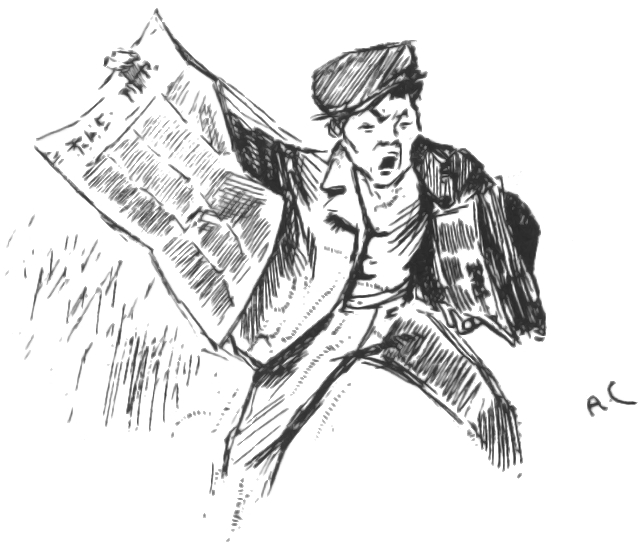
\includegraphics[width=0.5\textwidth]{2tailpiece}
%\captionlistentry{Tailpiece to Chapter \thechapter}
\end{wrapfigure}

Of course the two were quite unable to do anything. They shouted consolation and promises, and went off back to the town again to get help. One can imagine them, covered with sand, excited and disordered, running up the little street in the bright sunlight just as the shop folks were taking down their shutters and people were opening their bedroom windows. Henderson went into the railway station at once, in order to telegraph the news to London. The newspaper articles had prepared men's minds for the reception of the idea.

By eight o'clock a number of boys and unemployed men had already started for the common to see the »dead men from Mars.« That was the form the story took. I heard of it first from my newspaper boy about a quarter to nine when I went out to get my \textit{Daily Chronicle}. I was naturally startled, and lost no time in going out and across the Ottershaw bridge to the sand-pits.

%\begin{figure}[b!]
%\centering
%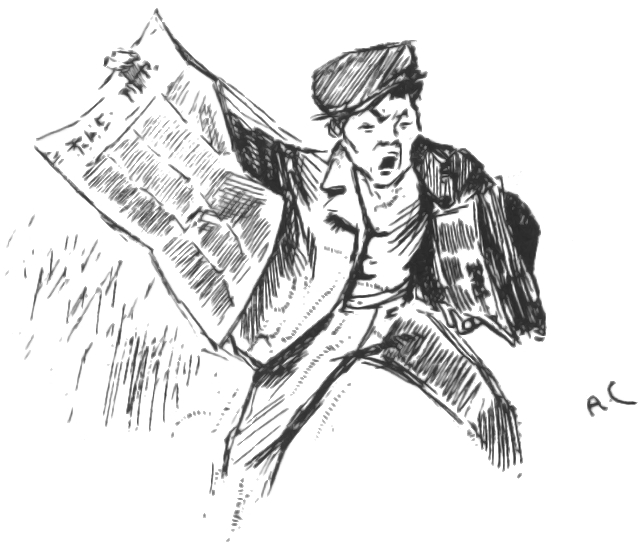
\includegraphics[width=.4\textwidth]{2tailpiece}
%\captionlistentry{Tailpiece to Chapter \thechapter}
%\end{figure}